% day01.tex

% Copyright 2019 Clara Eleonore Pavillet

% Author: Clara Eleonore Pavillet
% Description: This is an unofficial Oxford University Beamer Template I made from scratch. Feel free to use it, modify it, share it.
% Version: 1.0

\documentclass{beamer}
\setbeamertemplate{caption}[numbered]
\usepackage{import} % for some reason, this doesn't work when called in sty file
% Load Packages
\usepackage[utf8]{inputenc}
\usepackage{xcolor}
\usepackage{tikz}
\usetikzlibrary{positioning,calc}
\usepackage{graphicx}
\usepackage{hyperref}
\usepackage{amsmath}
\usepackage{listings}
\usepackage{fontawesome}

% Define Commands
\newcommand*{\ClipSep}{0.06cm} %To adjust footer logo
\newcommand{\E}{\mathrm{e}\,} %\def\I{e} % used to defined e for exp(x), see later what it should be
\newcommand{\ud}{\mathrm{d}}
\lstset{numbers=left, numberstyle=\tiny, stepnumber=1,firstnumber=1,breaklines=true,
    numbersep=5pt,language=Python,
    stringstyle=\ttfamily,
    basicstyle=\footnotesize, 
    showstringspaces=false
}

\usepackage{lecture_notes}
\usepackage{bibentry}
\usepackage[utf8]{inputenc}
\usepackage[T1]{fontenc}

% for manual multicolumns
\usepackage{multicol}
\setlength{\columnseprule}{1pt}
\def\columnseprulecolor{\color{black}}

% for embedded code (i.e., .bib reference)
\usepackage{listings}

\graphicspath{ {../../images/} }

\nobibliography*
% \usepackage[perpage]{footmisc}
\usetheme{oxonian}


\title{Day 03: \LaTeX Templates (CV and Beamer)}
\titlegraphic{
\includegraphics[width=3cm]{Theme/Logos/DavisLogoV1.png}}
\author{\small{Mason del Rosario}}
\institute{\LaTeX 101}
\date{September 2021} %\today

\begin{document}

\footnotesize{
% \bibliographystyle{ieeetr}
% \nobibliography*{refs}


{\setbeamertemplate{footline}{} 
\frame{\titlepage}}

  \section*{Course Recap}

  \begin{frame}{Course Recap}
    \begin{itemize} 
      \item \textbf{Adapted from} -- https://www.learnlatex.org/. 
        \begin{itemize}
          \item Day 1 -- \texttt{learnlatex.org} lessons 1-6 (\textbf{Done!})
          \item Day 2 -- \texttt{learnlatex.org} lessons 7-12 (\textbf{Done!})
          \item Day 3 -- \LaTeX templates (CV/resume, beamer presentations).
        \end{itemize}
      \item \textbf{Slides Available} -- https://github.com/mdelrosa/latex-101.
      \begin{itemize}
        \item Template based on \href{https://www.overleaf.com/latex/templates/oxpav/xnjgrxthvjhg}{Clara Pavillet's Oxford Template}
      \end{itemize}
      \item \textbf{Slack back channel}
      \begin{itemize}
        \item \href{https://join.slack.com/share/zt-ul82okyc-SI2GftuwPx_lFyBXll9rjw}{UC Davis Slack channel}
      \end{itemize}
    \end{itemize}
  \end{frame}

  \section*{Outline}\begin{frame}{Outline}\tableofcontents\end{frame}

  \section{Figures}

  \begin{frame}[plain]
    \vfill
    \centering
    \begin{beamercolorbox}[sep=8pt,center,shadow=true,rounded=true]{Graphics}
      \usebeamerfont{title}\insertsectionhead\par%
      \color{davisblue}\noindent\rule{10cm}{1pt} \\
      \footnotesize{Including images, resizing, positioning}
    \end{beamercolorbox}
    \vfill
  \end{frame}

  \nofoot{
  \begin{frame}{Templates}
    \begin{itemize}
      \item Writing documents from scratch is time-consuming, difficult.
      \item Instead, use templates!
    \end{itemize}
    \begin{figure}
      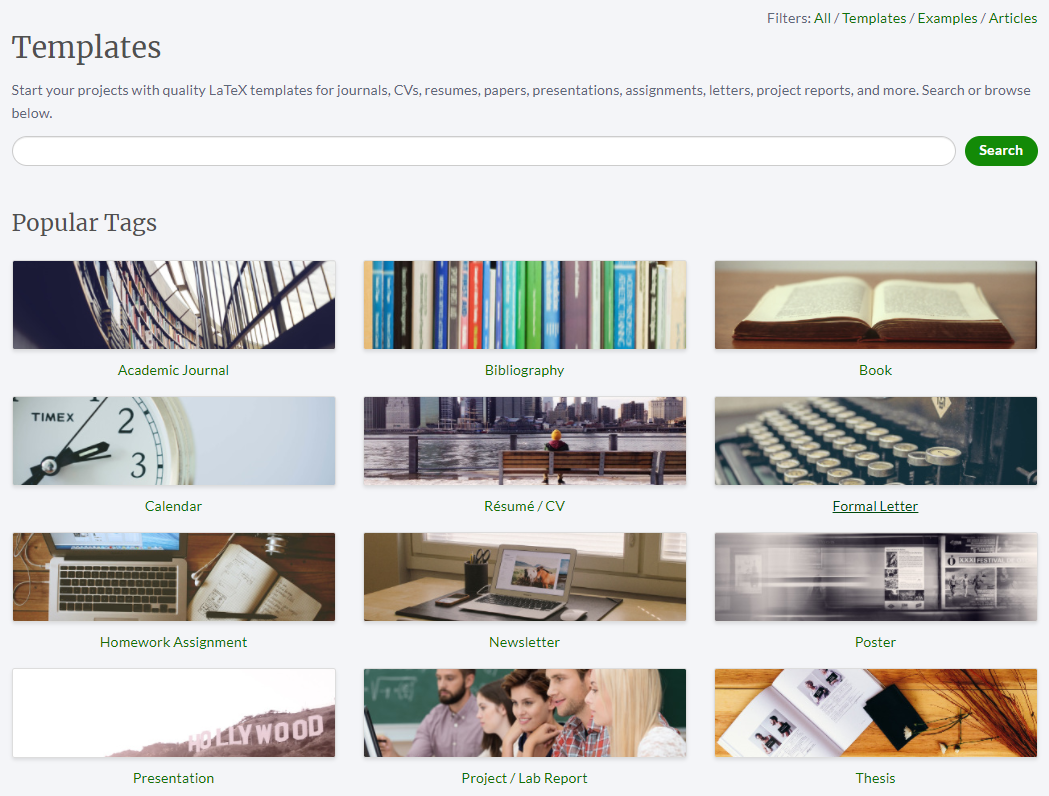
\includegraphics[width=0.7\linewidth]{day03-00-templates.png}
      \caption{Template categories on Overleaf.}
      \label{fig:day03-00-templates}
    \end{figure}
  \end{frame}
  }

  \nofoot{
  \begin{frame}{Templates}
    For academic journals, some official templates are available.
    \begin{figure}
      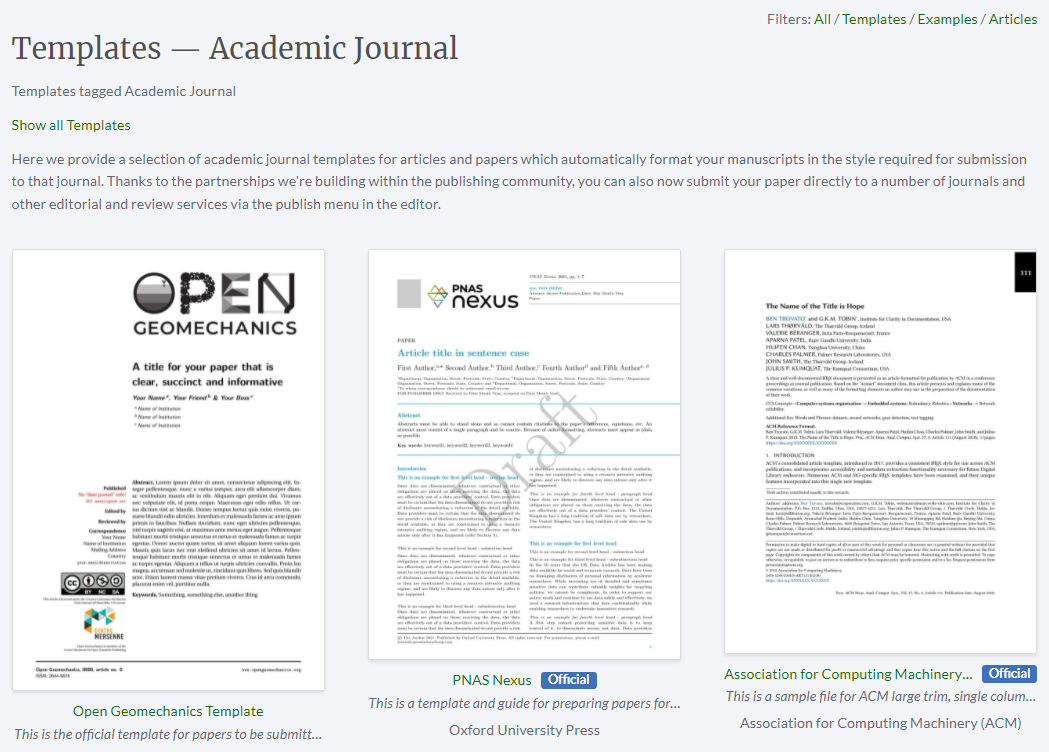
\includegraphics[width=0.7\linewidth]{day03-01-official.png}
      \caption{Academic journal templates on Overleaf.}
      \label{fig:day03-01-official}
    \end{figure}
  \end{frame}
  }

\begin{frame}{End of Day 02}
  \begin{itemize}
    \item Finished: Lessons 1-6 (Day 01) and 7-12 (Day 02) from \texttt{learnlatex.org}
    \item Lessons 13 to 16 -- can ask questions re: these on the Slack channel! (\#latex101)
    \item Next time: Resume/CV templates, Beamer, Inkscape
  \end{itemize}
\end{frame}

\begin{frame}{References}
  \bibliographystyle{ieeetr}
  \bibliography{example}
\end{frame}

} %end footnotsize

\end{document}
